\chapter{Sviluppo}
In questo capitolo verrà descritto il processo di sviluppo
seguito per l'implementazione di \pygfa, analizzandone le
fasi principali, descrivendo i problemi incontrati e come sono stati
affrontati.

\section{Processo}
Lo scopo di \pygfa è quello di fornire un ambiente per lo sviluppo
di applicativi in grado di analizzare e manipolare file GFA. Non
è pertanto un prodotto finito, con casi d'uso definiti e risultati attesi
con cui è possibile confrontare i risultati. Non si è ritenuto appropriato,
di conseguenza, seguire un processo di sviluppo con fasi di analisi
e pianificazione profonde, che con il mutare dei requisti (per la
maggior parte non definiti fin dall'inizio) avrebbero potuto
compromettere la struttura del sistema. Un altro fattore da
tenere in considerazione è che le mie conoscenze sul significato
che i dati contenuti nei file GFA e le considerazioni che si potevano dedurre
da esse sono cresciute con lo sviluppo del sistema stesso. Perciò un'analisi,
anche se non approfondita, non poteva essere svolta a priori; poiché
avrebbe potenzialmente comportato una serie di ritardi
nello sviluppo del progetto dovute allo studio di concetti biologici che
avrebbero richiesto un periodo di studio non trascurabile.

Per questi motivi, il processo di sviluppo che si è deciso di utilizzare è di \emph{extreme}
\emph{programming}; con fasi di analisi e pianificazione molto veloci,
dando priorità all'implementazione delle parti essenziali del sistema aventi
maggior priorità per poi ripetere il procedimento con l'evolversi dei
requisiti e delle funzionalità richieste, cercando di avere un riscontro
costante con i clienti finali (in questo caso i referenti della tesi).

Affiancata alla parte di implementazione si è svolta la parte di testing,
che purtroppo non si è riusciti a condurre esattamente nella forma di Test Driven
Development, ma alla quale è stata data comunque una priorità molto alta
sia per la verifica delle funzionalità dei metodi, che per la verifica della
presenza di errori nel codice, che nel contesto di un linguaggio non compilato
quale è il Python, risulta una pratica molto importante per garantire il
corretto funzionamento del programma.

Nel complesso si è riusciti a seguire abbastanza rigorosamente questi cicli
di pianificazione veloce, implementazione e test; procedendo al termine
di ogni ciclo con una fase di refactoring del codice e di miglioramento
della documentazione presente in esso, avvalendosi di Pylint per individuare
quelle porzioni di codice che era possibile migliorare.

\subsection{Fasi di sviluppo}
\'E possibile suddividere lo sviluppo di \pygfa in tre fasi principali:
\begin{itemize}
	\item sviluppo del parser;
	\item progettazione delle classi di astrazione dei dati GFA;
	\item sviluppo della classe del grafo GFA e delle operazioni che è
		possibile eseguire su di esso.
\end{itemize}
\captionsetup{justification=centering}
\begin{figure}[h]
	\centering
	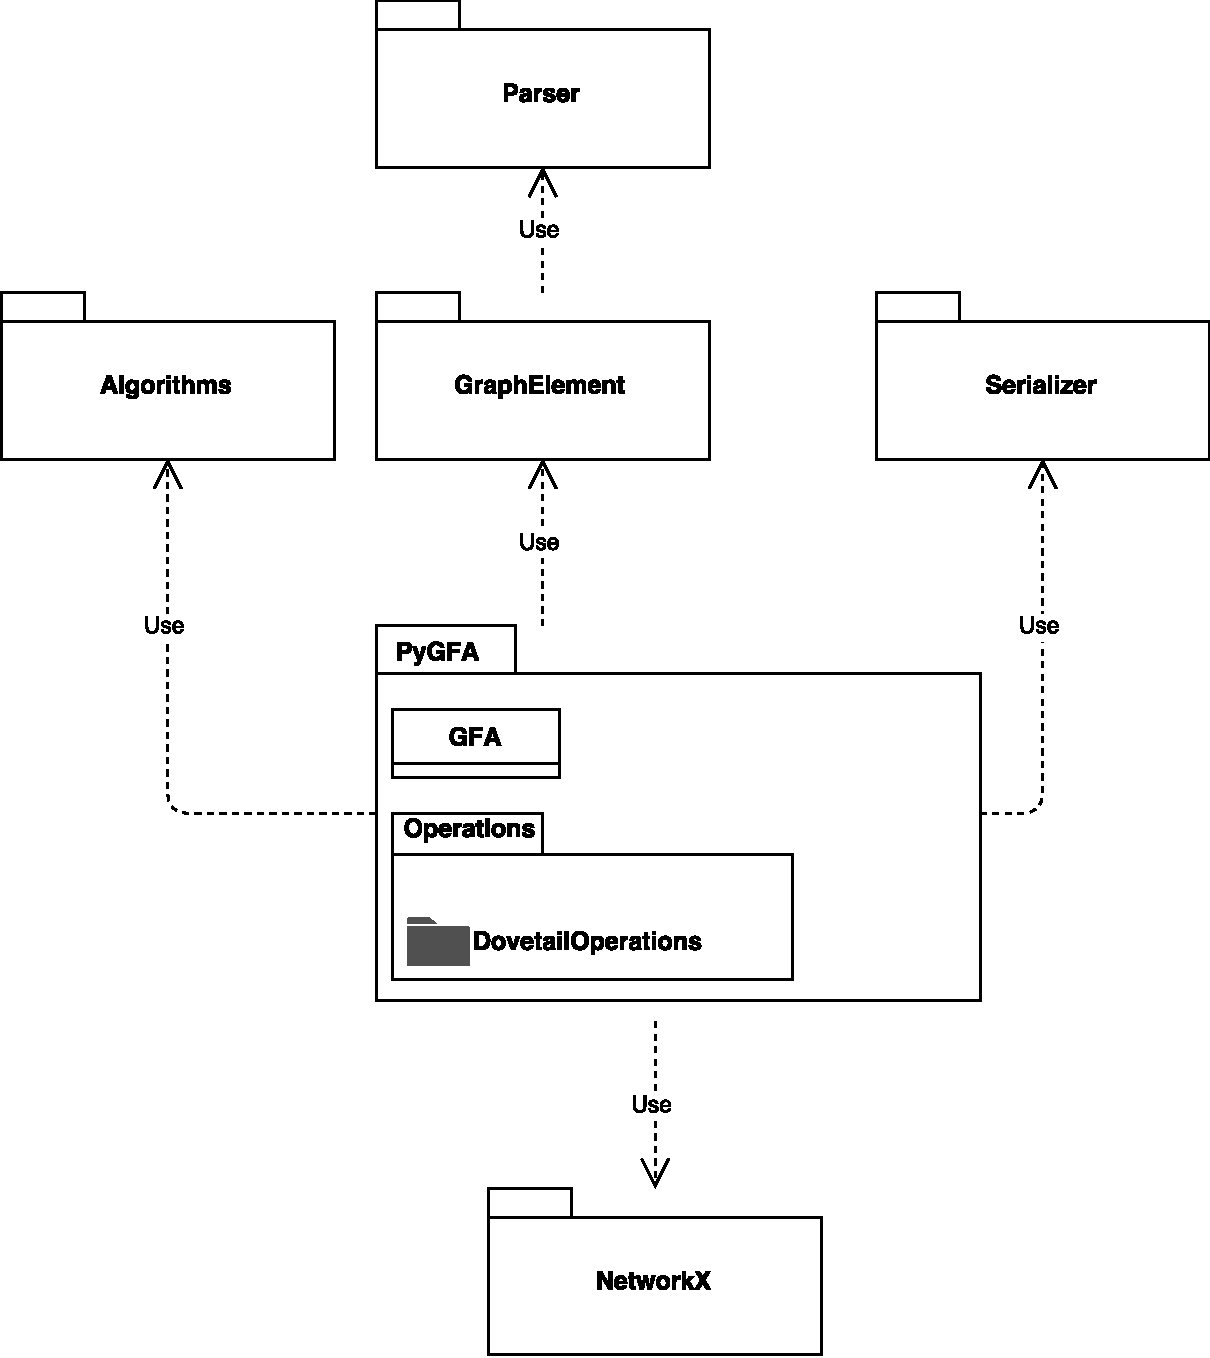
\includegraphics[scale=0.5]{package_diagram}
	\caption[Diagramma dei package]{Diagramma dei package di \pygfa.}
\end{figure}
\captionsetup{justification=justified}

Il parser si occupa di leggere le linee di un file GFA, di verificare la correttezza
sintattica dei suoi campi e di rappresentarne le informazioni mediante una classe
specifica per ogni tipo di linea.

Nella seconda fase si sono analizzate le linee delle due specifiche e si
è stabilito come attribuire ad ogni linea un ruolo che potesse essere di
nodo, arco o sottografo del grafo GFA finale. Gli attributi delle classi
del grafo astraggono gli attributi delle linee delle specifiche, 
di conseguenza è stata necessaria
una pianificazione dell'assegnamento degli attributi delle linee ad
attributi degli elementi del grafo.

Nella fase finale si è sviluppata la classe del grafo GFA fornendo
metodi di inserimento, accesso ed eliminazione sui singoli elementi che
lo compongono e aggiungendo le interfacce agli algoritmi forniti da Networkx
per eseguire le operazioni sui dati GFA.

\section{Fase1: sviluppo del parser}
Per la scrittura del parser si è seguito un approccio \emph{bottom-up},
sviluppando dapprima le classi rappresentanti i campi,
che sono presenti in ogni linea, 
e successivamente descrivendo con una classe ciascun tipo
di linea presente nelle specifiche.

Il parser effettua solo un controllo sintattico sulle informazioni dei file
al fine di garantire una corretta gestione delle informazioni da parte
della libreria; non verifica eventuali incongruenze tra le informazioni
presenti. Per questo motivo si suppone che il file GFA che viene fornito
sia stato già validato da un punto di vista di namespace degli elementi
e di coerenza delle informazioni (per esempio il riutilizzo di un identificativo
già utilizzato da un altro elemento o la descrizione di linee e segmenti
che non vengono definiti).

Ogni campo di ogni linea, in entrambe le specifiche, può essere descritto
da un \emph{espressione regolare}. Per questo motivo è stato
implementato un modulo Python per la validazione di tutti i campi definiti
dalle specifiche,
associando un nome ad ogni espressione e creando un metodo
\texttt{is\_valid} che, data una stringa e il nome del tipo di un campo,
verifica che la stringa rispetti l'espressione regolare indicata dal nome
del campo fornito.

Per rappresentare i campi delle linee sono state create due classi,
\texttt{Field} e \texttt{OptField}, rispettivamente. La prima
descrive i campi obbligatori, per i quali non viene specificato
esplicitamente il tipo di dato che contengono, i secondi aventi
nome (il tag), tipo e valore. Mentre nei campi opzionali
è possibile, fin dall'instanziazione dell'oggetto, effettuare una validazione
sul contenuto, sui campi obbligatori non è possibile, in quanto
la tipologia del loro contenuto assume valore solo nel contesto
della linea cui appartengono.



